\maketitle
\setcounter{page}{1}
\tableofcontents
\newpage
\pagenumbering{arabic}
\section{Theorie}
Der Zeeman-Effekt tritt auf, wenn Atome einem externen Magnetfeld unterworfen
werden. Dadurch wird die Entartung der Energieniveaus in der Quantenzahl $m$
aufgehoben, sodass die diese Energieniveaus aufspalten. \\
\\
Zur Berechnung der Wechselwirkung der Drehimpulse und der magnetischen Momente
untereinander, müssen die Drehimpulse eines Hüllenelektrons betrachtet werden, also
der Bahndrehimpuls $\vec{l}$ und der Spin $\vec{s}$. Das magnetische Moment
des Drehimpulses ist definiert nach
\begin{equation}
  \vec{\mu}_l = -\mu_B \, \frac{\vec{l}}{\hbar} = -\mu_B \, \sqrt{l(l+1)} \ \vec{l}_e
  \label{eqn:1}
\end{equation}
mit dem magnetischen Moment
\begin{equation*}
  \mu_B = -\frac{1}{2} \, \symup e_0 \, \frac{\hbar}{\symup m_0} \, ,
\end{equation*}
dem Einheitsvektor $\vec{l}_e$ in $\vec{l}$ Richtung und mit Elementarladung und
Ruhemasse des Elektrons.
Aus dem Spin-Gerlach-Experiment folgt das Analogon für den Spin
\begin{equation}
  \vec{\mu}_s = - \symup g_s \, \frac{\mu_B}{\hbar} \, \vec{s}
  = - \symup g_s \, \mu_B \, \sqrt{s(s+1)} \ \vec{s}_e
  \label{eqn:2}
\end{equation}
mit dem \textsc{Landé-Faktor} des Elektrons $\symup g_s$, welcher ungefähr den
Wert 2 besitzt. Wie aus \eqref{eqn:1} und \eqref{eqn:2} ersichtlich, ist damit
$\vec{\mu}_s$ entwa doppelt so groß wie $\vec{\mu}_l$. Dies wird als \textbf{magnetomechanische
Anomalie des Elektrons} bezeichnet. Nun werden, wie bereits erwähnt, die Wechelwirkungen
der Drehimpulse und magnetischen Momente untereinander und miteinander behandelt.
Da diese aber im Allgemeinen sehr unübersichtlich sind, werden zwei Grenzfälle betrachtet:
\begin{itemize}
  \item \textbf{Niedrige Kernladungszahl}:
  Die Wechselwirkung zwischen den Bahndrehimpulsen ist so dominant, dass sich
  durch Addition ein Gesamtdrehimpuls $\vec{L}$ der Hülle aus diesen bildet. Die
  Bahndrehimpulse von abgeschlossenen Schalen sind dabei stets 0 und fließen somit
  nicht in den Gesamtdrehimpuls ein. $\vec{L}$ ist dabei quantisiert, und zwar
  gibt es nur Gesamtdrehimpulse, deren Quantenzahl ganzzahlig ist. Die Terme zu den
  Quantenzahlen 0, 1, 2 und 3 heißen S-, P-, D- und F-Terme. Der Gesamtdrehimpuls
  hat ebenfalls ein zugehöriges magnetisches Moment, welches sich aus \eqref{eqn:1}
  zu
  \begin{equation}
    |\vec{\mu}_L| = \mu_B \, \sqrt{L(L+1)}
    \label{eqn:3}
  \end{equation}
  ergibt. Auch für den Spin gibt es einen Gesamtspin, analog zum Bahndrehimpuls,
  mit dem Unterschied, dass für die Quantisierung $\frac{N}{2}, \frac{N}{2} - 1, ...,
  \frac{1}{2}, 0$ (Mit $N$ als Gesamtzahl der Elektronen in unabgeschlossenen Schalen) gilt.
  Analog zu \eqref{eqn:3} gilt für das magnetische Moment des Gesamtspins
  \begin{equation}
    |\vec{\mu}_s| = \symup g_s \mu_B \, \sqrt{S(S+1)} \, .
    \label{eqn:4}
  \end{equation}
  Unter der Vorraussetzung, dass das angelegte externe Magnetfeld kleiner als ungefähr
  \SI{10}{\tesla}, koppeln Gesamtspin $\vec{S}$ und Gesamtdrehimpuls $\vec{L}$ zum Gesamtdrehimpuls
  $\vec{J} = \vec{L} + \vec{S}$ der Elektronenhülle. Dies nennt sich \textbf{LS-Kopplung}.
  Für den Versuch wird diese Kopplungsart angenommen. Die Quantenzahl des Gesamtdrehimpulses
  ist entweder halb- oder ganzzahlig, abhängig von S.
  \item \textbf{Hohe Kernladungszahl}:
  In diesem Fall ist die Wechselwirkung zwischen Spin und Bahndrehimpuls eines
  Elektrons dominant gegenüber der Wechselwirkung der Größen untereinander. Somit
  existiert kein Gesamtdrehimpuls und Gesamtspin, lediglich der Gesamtdrehimpuls
  \begin{equation*}
    \vec{J} = \sum_i \ \vec{l}_i + \vec{s}_i
  \end{equation*}
  der Hülle existiert noch.
\end{itemize}
Nun wird die Aufspaltung der Energieniveaus näher betrachet. Als erstes wird das
magnetische Moment zum Gesamtdrehimpuls $\vec{J}$
\begin{equation}
  \vec{\mu} = \vec{\mu}_L + \vec{\mu}_S
  \label{eqn:5}
\end{equation}
definiert. Die senkrechte Komponente des magnetischen Moments (relativ zu $\vec{J}$)
verschwindet dabei. Für den Betrag des magnetischen Moments ergibt sich
\begin{equation}
  |\vec{\mu}_J| = \mu_B \, \symup g_J \, \sqrt{J(J+1)} \, .
  \label{eqn:6}
\end{equation}
Dabei gilt
\begin{equation}
  \symup g_J = \frac{3 \, J(J+1) + S(S+1) - L(L+1)}{2 \, J(J+1)}
  \label{eqn:7}
\end{equation}
für den sogenannten \textbf{Landé-Faktor}. Weiterhin ist zu beachten, dass sich
nach Anlegen eines externen Magnetfeldes nur solche Winkel zwischen $\vec{mu}$ und
$\vec{B}$ ein, bei denen
\begin{equation*}
  \mu_{J_z} = - m \, g_J \, \mu_B
\end{equation*}
für die z-Komponente des magnetischen Moments gilt. Dabei ist $m$ die bereits oben
erwähnte \textbf{Orientierungsquantenzahl}, die von $-J, -J + 1, ..., J$ definiert ist.
Nun lässt sich über $E_\symup{mag} = - \vec{\mu}_J \cdot \vec{B}$ die Energie berechnen,
die das magnetische Moment im Magnetfeld erhält. Mit \eqref{eqn:7} folgt
\begin{equation}
  E_\symup{mag} = m \, \symup g_J \, \mu_B \, .
  \label{eqn:8}
\end{equation}
Mit \eqref{eqn:8} ist nun ein Ausdruck für die Aufspaltung der Energieniveaus
in äquidistante Niveaus gegeben. Da dies nicht nur auf den Grundzustand, sondern
auch auf alle angeregten Zustände zutrifft, wird es neue Übergänge zwischen den
Energieniveaus geben, welche sich in der Aufspaltung der Spektrallinien äußert. \\
\\
Zur Bestimmung der Auswahlregeln für Übergänge zwischen den neu entstandenen Energieniveaus
wird die zeitabhängige Schrödingergleichung gelöst. Als Lösung für die Wellenfunktion
wird eine Linearkombination aus zwei Lösungen für die an dem Übergang beteiligten
Energieniveaus genutzt, die da lautet
\begin{equation*}
  \Psi_\symup{ges}(\vec{r}, t) = C_\alpha \,  \Psi_\alpha(\vec{r}) \, \symup{exp}
  \left(-\frac{\symup i}{\hbar} \, E_\alpha \, t \right) +
  C_\beta \, \Psi_\beta(\vec{r}) \, \symup{exp}
  \left(-\frac{\symup i}{\hbar} \, E_\beta \, t \right)
\end{equation*}
mit $C_{\alpha, \beta}$ als Koeffizienten, die man aus der Normierbarkeit erhält
und $E_{\alpha, \beta}$ als Energieniveaus,
zwischen denen der Übergang stattfindet. Im folgenden werden über die Intensität
der emittierten Strahlung mittels Poyting-Vektor die Auswahlregeln
\begin{equation}
  \symup \Delta m = 0, -1 \ \text{und} \ +1
  \label{eqn:9}
\end{equation}
mit $\symup \Delta m = |m_\alpha - m_\beta|$, also der Differenz der Orientierungsquantenzahlen
der beiden Niveaus. Bei $\symup \Delta m = 0$ ist die emittierte Strahlung linear
zu $\vec{B}$ polarisiert. Bei $\symup \Delta m = \pm 1$ eine in der Drehrichtung
unterschiedliche zirkulare Polarisation zu erkennen. \\
\\
Da in der zeitabhängigen Schrödingergleichung der Spin nicht berücksichtigt wird,
sind die bisherigen Ergebnisse nur für den Fall $S = 0$ gültig. Dies nennt man den
\textbf{Normalen Zeeman-Effekt}. In diesem Fall gilt nach \eqref{eqn:7} für
alle $J$: $g_J = 1$. Folglich sind die Aufspaltungen unabhängig von den Quantenzahlen.
\begin{figure}
  \centering
  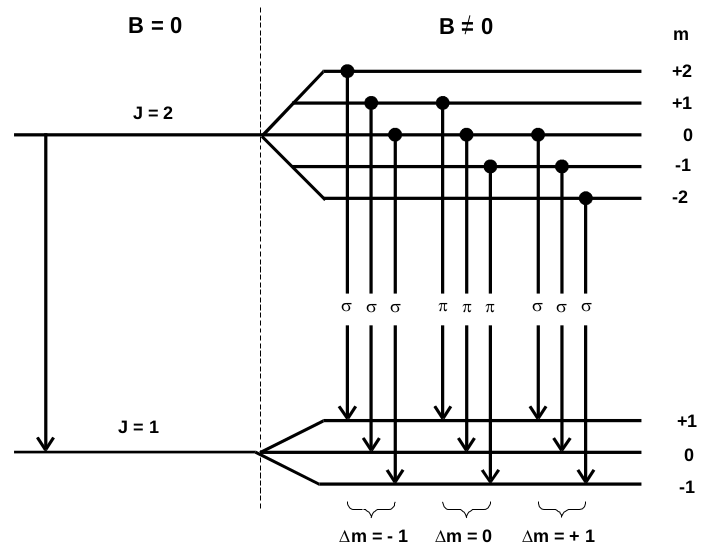
\includegraphics[scale=0.4]{normal.png}
  \caption{Aufspaltung der Energieniveaus und zugehörige Polarisation für den
  normalen Zeeman-Effekt. \cite{anleitung}}
  \label{fig:1}
\end{figure}
Ein Beispiel für eine solche Aufspaltung ist in Abbildung \ref{fig:1} zu sehen.
Dabei ist zu sehen, dass die Energieniveaus äqudistant sind. Dies folgt aus \eqref{eqn:8},
da $g_J = 1$ gilt. Es ergibt sich
\begin{equation}
  E_\symup{mag}= m \, \mu_B \, B \, .
  \label{eqn:10}
\end{equation}
Die Aufspaltungslinien lassen sich den Auswahlregeln zuordnen, was auch in
Abbildung \ref{fig:1} dargestellt ist. Allerdings sind je nach Beobachtungsrichtung
wegen der unterschiedlichen Polarisation nicht alle Linien zu sehen. Die $\pi$-Linie
(zu $\symup \Delta m = 0$) ist nur sichtbar, wenn die Beobachtungsrichtung
senkrecht zur Feldrichtung, also transversal, ist. Außerdem ist sie gegenüber
der feldfreien Linie nicht verschoben, im Gegensatz zu den Linien mit $\symup \Delta m = \pm 1$,
da sich die Energie um $\mu_B \, B$ im Vergleich zum feldfreien Fall unterscheidet.
Weil sie zirkular polarisiert sind, erscheinen sie bei transversaler Beobachtung als
linear polarisiert. So eine Aufspaltung ist in Abbildung \ref{fig:2} zu sehen.
\begin{figure}
  \centering
  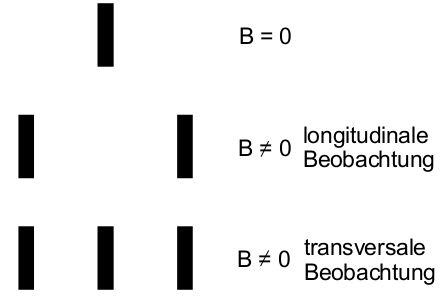
\includegraphics[scale=0.5]{normal2.png}
  \caption{Aufspaltung einer Spektrallinie nach Beobachtungsrichtung beim
  normalen Zeeman-Effekt.}
  \label{fig:2}
\end{figure}
Der andere Fall, also $S \neq 0$, wird \textbf{Anormaler Zeeman-Effekt} genannt.
Die Auswahlregeln \eqref{eqn:9} sind auch in diesem Fall noch gültig, dies lässt
sich über die spinabhängige Schrödingergleichung zeigen. Die Auspaltung wird
vielfältiger, da $g$ nicht mehr für alle $J$ 1 ist, sondern von $L, S$ und $J$
abhängt.

\section{Durchführung}
\subsection{Versuchsaufbau}
\begin{figure}
  \centering
  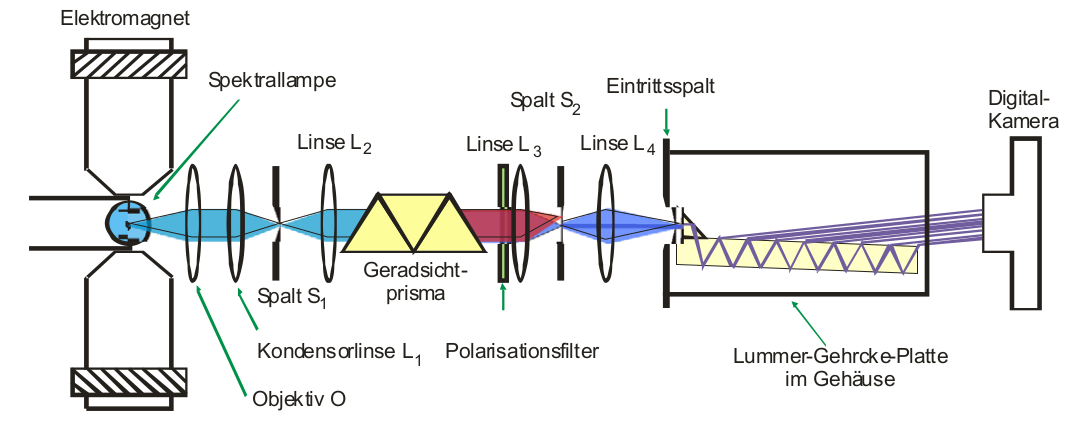
\includegraphics[scale=0.38]{aufbau.png}
  \caption{Der Versuchsaufbau im Schema.}
  \label{fig:3}
\end{figure}
Der Aufbau des Versuchs ist in Abbildung \ref{fig:3} zu sehen. Das Licht stammt
von einer Cd-Lampe, deren rote und blaue Linie aufgespalten werden. Dies wird realisiert,
indem die Lampe in einen starken Elektromagnet gestellt wird. Dann wird transversal
zum Magnetfeld durch Linsen, Spalte und ein Geradsichtprisma das Licht nach Wellenlängen
aufgespalten. Nun kann durch eine Spalt und einen Polarisationsfilter die gewünschte
Linie mit der gewünschten Polarisation ausgewählt und auf eine Lummer-Gehrke-Platte
abgebildet werden. Das entstehende Interferenzmuster wird über eine Digitalkamera
aufgenommen. Bei monochromatischem Licht erzeugt die Lummer-Gehrke-Platte Gangunterschiede
von $\lambda$, also genau der eingestrahlten Wellenlänge. Durch Einschalten des Magnetfeldes
tritt eine Verschiebung der Wellenlänge um $\delta \lambda$ auf, welche wiederum
die interferierten Straheln um $\delta s$ verschiebt. Dabei ist allerdings zu beachten,
dass das Dispersionsgebiet
\begin{equation}
    \symup \Delta \lambda_D = \frac{\lambda^2}{2\, d} \cdot \sqrt{\frac{1}{n^2 - 1}}
    \label{eqn:11}
\end{equation}
nicht überschritten wird, da sonst eine Überlagerung der Wellenlängen auftreten
(mit $d$ als Dicke der Platte und $n$ als Ordnung des Maximums). Für das
Auflösungsvermögen $A$ der Lummer-Gehrke-Platte gilt
\begin{equation}
  A = \frac{L}{\lambda} (n^2 - 1)
  \label{eqn:12}
\end{equation}
mit $L$ als Länge der Platte und $n$ als Brechungsindex.
\subsection{Versuchsdurchführung}
Zuerst wurde der Elektromagnet geeicht, indem das B-Feld über ein Gaussmeter
in Abhängigkeit vom Feldstrom gemessen wird in einem Intervall von $0 \leq I \leq \SI{20}{\ampere}$.
Dann wird der bereits beschriebene Aufbau so justiert, dass die gesuchten Wellenlängen
($\lambda = \SI{480}{\nano\meter}$ und $\lambda = \SI{643.8}{\nano\meter}$)
mit der durch den Polarisationsfilter eingestellten Polarisation auf die Lummer-Gehrke-Platte
fallen. Dann werden mittels Digitalkamera Bilder von Interferenzbildern bei verschiedenen Polarisationen
und Magnetfeldstärken aufgenommen, um daraus die Wellenlängenverschiebung zu bestimmen.

\section{Auswertung}
\subsection{Eichung des B-Feldes}
Die Messwerte sowie eine graphische Darstellung mit Fit sind in Abbildung \ref{A_Abb:1}
dargestellt. Der Fit wurde nach least-squares durch die Funktion $\textsc{polyfit}$
aus dem $\textsc{Python}$\footnote{Version: 3.6.3} Paket
$\textsc{numpy}$\footnote{Version: 1.13.3} mit einem Polynom 3. Grades erstellt.

\begin{figure}[h!]
  \centering
  \subcaptionbox{Messwerte.}[0.20\textwidth]{
  \centering
  \begin{tabular}{c c}
    \toprule
    $I / \si{\ampere}$ & $B / \si{\milli\tesla}$ \\
    \midrule
    0 & 5 \\
    1 & 64 \\
    2 & 139 \\
    3 & 191 \\
    4 & 237 \\
    5 & 308 \\
    6 & 363 \\
    7 & 423 \\
    8 & 486 \\
    9 & 533 \\
    10 & 599 \\
    11 & 662 \\
    12 & 720 \\
    13 & 770 \\
    14 & 821 \\
    15 & 870 \\
    16 & 915 \\
    17 & 949 \\
    18 & 985 \\
    19 & 1006 \\
    20 & 1032 \\
    \bottomrule
  \end{tabular}
  }
  \subcaptionbox{Grafische Darstellung mit Regression.}[0.78\textwidth]{
  \centering
  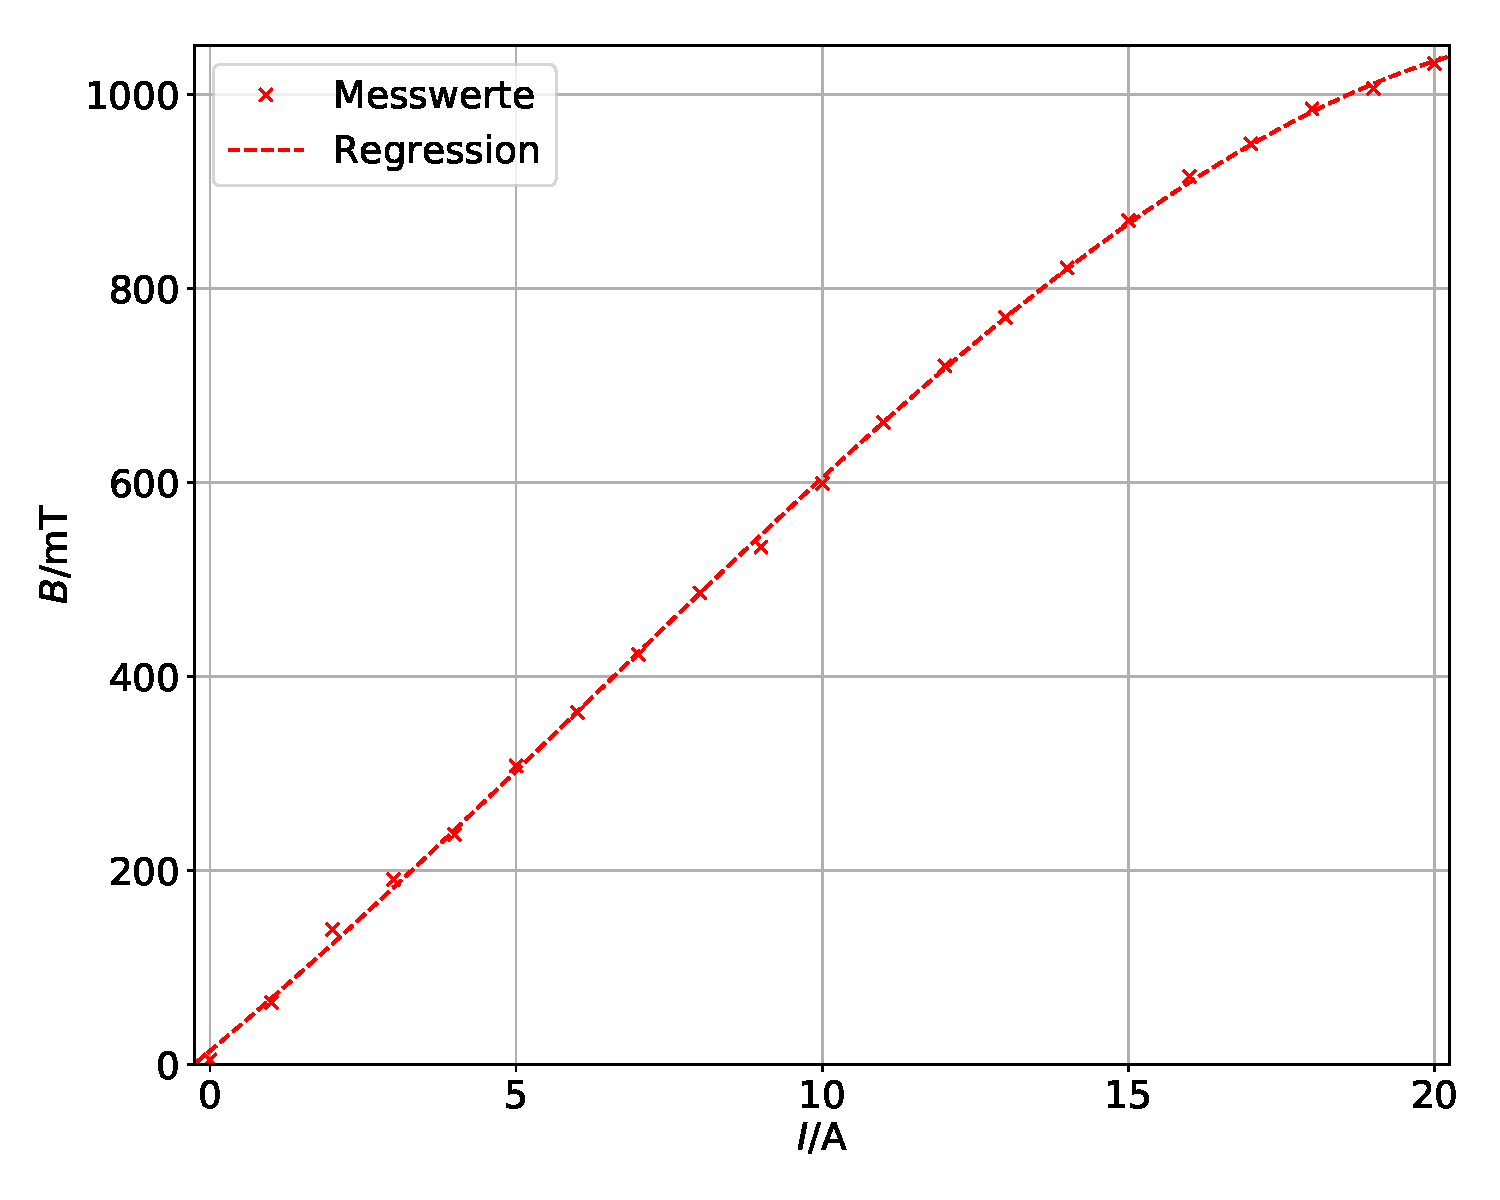
\includegraphics[width=0.78\textwidth]{B_Feld.pdf}
  }
  \caption{Magnetfeldeichung.}
  \label{A_Abb:1}
\end{figure}

Die Fitparameter mit Fehlern lauten:
\begin{align}
\begin{split}
  a_3 &= \SI{-0.072(9)}{\milli\tesla\per\cubic\ampere}\\
  a_2 &= \SI{1.350(269)}{\milli\tesla\per\square\ampere}\\
  a_1 &= \SI{52.760(2284)}{\milli\tesla\per\ampere}\\
  a_0 &= \SI{14.007(5145)}{\milli\tesla}.
  \label{A_eq:1}
\end{split}
\end{align}
Mit den Werten in \eqref{A_eq:1} folgt also als genäherte Feldstromstärke - Magnetfeld
- Beziehung:
\begin{equation}
  B(I) = a_3 \cdot I^3 + a_2 \cdot I^2 + a_1 \cdot I + a_0
\end{equation}



\newpage
\nocite{*}
\printbibliography
